\section{Introduction}

Natural Language Processing (NLP) has witnessed rapid progress in recent years driven by the attention mechanism~\cite{46201}. 
Attention models such as Transformer~\cite{46201}, \bert~\cite{devlin2018bert}, and \gpttwo~\cite{radford2019language} provide significant performance improvements over models based on Convolutional Neural Networks (CNN) and Recurrent Neural Networks (RNN). \bert~\cite{devlin2018bert} even outstrips human performance on the challenging sentence classification~\cite{wang-etal-2018-glue} tasks. 

Unfortunately, the high accuracy is at the expense of efficiency. Attention runs extremely slow on general-purpose platforms, due to its quadratic computational complexity to input length, complex data movement and low arithmetic intensity. 
For instance, to generate a sentence with only 30 tokens, a \gpttwo model takes a total of 370ms on a \titanxp \xspace to perform attention inference. That is two orders of magnitude slower than MobileNet-V2, which takes only 6ms to classify an image. 
On resources-limited \rasp, attentions cost 43s, making interactive dialog applications impossible. The inefficiency is even more severe for modern Large Language Models (LLMs) with long context length and large KV cache.
The efficiency barrier prevents attention models from being deployed on mobile devices. 
Many accelerators have been proposed to accelerate CNN and RNN, but they cannot be easily applied to attention due to the distinct operations. 

\begin{figure}[t]
    \centering
    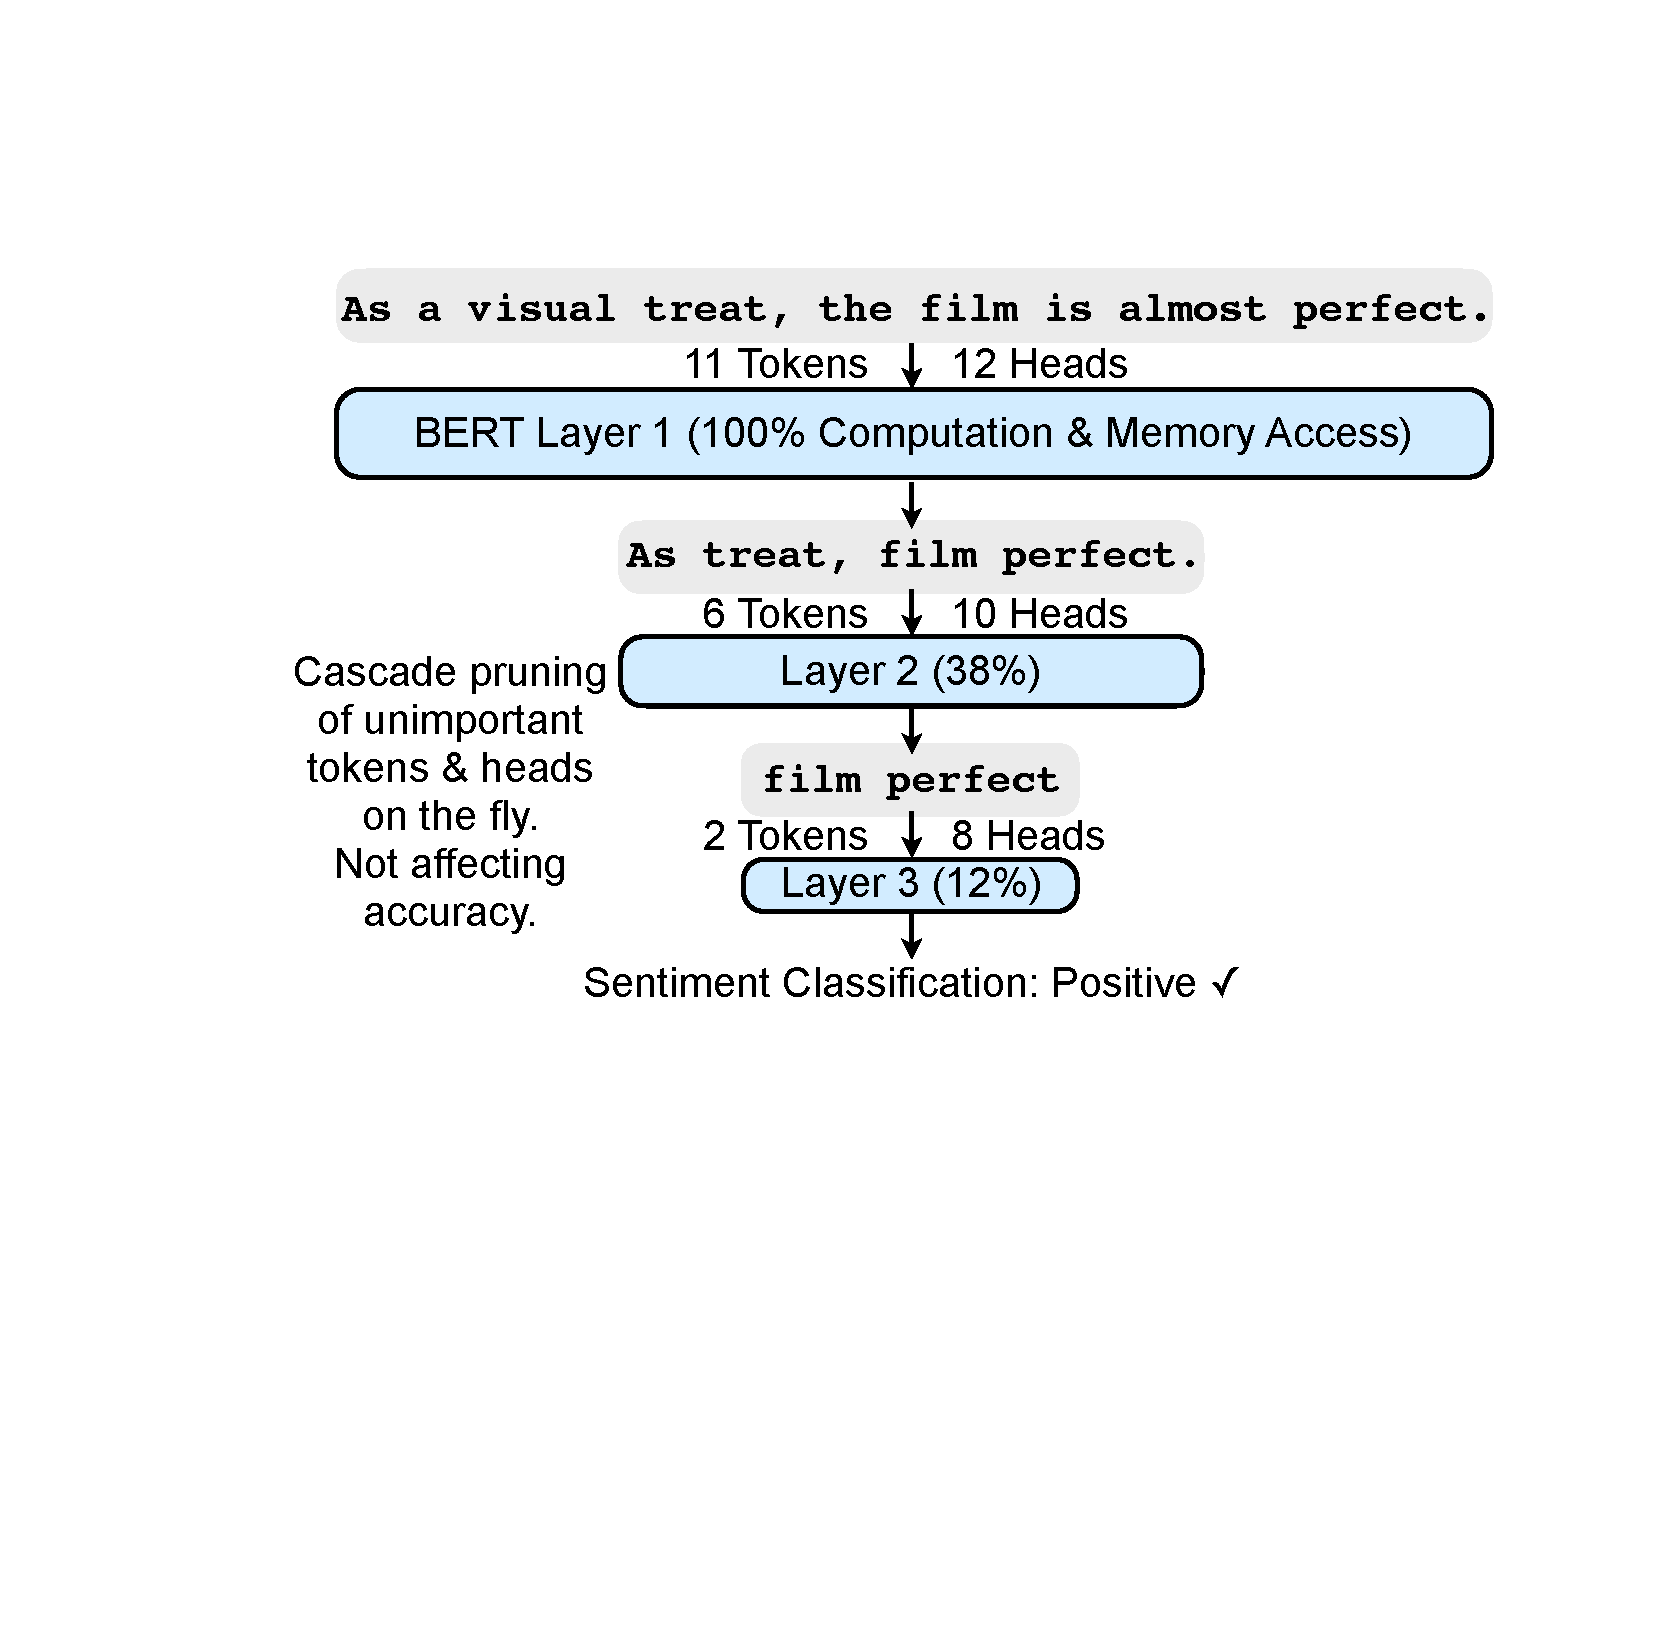
\includegraphics[width=\columnwidth]{figures/corrected-teaser.pdf}
    \vspace{-20pt}
    \caption{\textit{Cascade token and head pruning} removes redundant tokens and heads globally across layers. Evaluated with BERT-Base on SST-2 dataset.}
    \vspace{-10pt}
    \label{fig:teaser}
\end{figure}

In this paper, we propose \name\footnote{\name is homophonic with \emph{spartan}, meaning simple and frugal. It is analogous to \emph{token and head pruning}, making sentences shorter and simpler.}, an algorithm-architecture \codesign to enable efficient attention inference. We propose three algorithmic optimizations: \emph{cascade token pruning}, \emph{cascade head pruning} and \emph{progressive quantization} to reduce computation and memory access. Different from conventional techniques, pruning is applied to the tokens and heads, not weights. Cascade means: once a token/head is pruned, it is removed in all following layers, so one layer only needs to process remaining tokens/heads from previous layers. The deeper the layer, the more tokens/heads are pruned. The three techniques are input-dependent since the pruned computation and bit-width are \emph{adaptive} to input instances. Cascade pruning requires sorting token/head importance scores on the fly. Thus we design hardware architecture with high parallelism \topk engines for token/head selections, specialized memory hierarchy, and fully-pipelined datapath to translate theoretical savings to real speedup and energy reduction.


The inputs of attention contain Query (Q), Key (K), and Value (V), each split into multiple heads.
Then attention probabilities are computed as the softmax of Q $\times$ K. Multiplying the attention probabilities with V gives the result of one head; concatenating all heads together gives the attention output.
The arithmetic intensity of attention in the generation stage is low: only two operations per data (0.5ops/Byte) for the vector-matrix multiplication (Q $\times$ K). Generation takes the largest part of overall latency in \gpttwo models (97\% when generating 32 tokens); thus, the overall performance is memory-bounded. For \bert, the overall performance is computation-bounded.


Therefore, we propose \emph{cascade token pruning} as shown in Figure~\ref{fig:teaser} to reduce both DRAM access and computation. Inspired by human languages being highly redundant due to many structural and meaningless tokens such as prepositions, articles, and adverbs, we can safely remove unimportant tokens with little impact on the results. Moreover, attention uses many heads to capture various dependencies, but some of them are also redundant~\cite{voita2019analyzing}. Therefore, we also propose \emph{cascade head pruning} to determine the importance of heads based on their influence on the outputs, then prune unessential heads. Cascade token and head pruning are fundamentally different from the classic weight pruning and classic head pruning because: (i) There is no trainable weight in attention. (ii) Conventionally, pruned weights and heads are determined at compile-time and consistent for all inputs. In contrast, tokens and heads to be pruned in \name are selected on the fly and vary between different inputs. Token pruning is also different from classic activation pruning because it depends on attention probabilities, not activation magnitude. Specifically, we prune the tokens according to cumulative token importance scores obtained by accumulating attention probabilities (indicators for token influence) across layers. Since long sentences are naturally more redundant, we also adjust the pruning ratios based on sentence length: the longer, the more tokens are pruned away. Moreover, the heads are pruned according to cumulative head importance scores, which are computed by accumulating each head's magnitude across layers. 
To support cascade token and head pruning, we design and implement a specialized high parallelism \topk engine with $O(n)$ time complexity to get the $k$ most essential tokens or heads. On average, token and head pruning can reduce DRAM access and computation by \prunegpttwodramsaving\x and \hpdramsaving\x on eight \gpttwo models.

To further reduce the DRAM access, we also propose \emph{progressive \lowprec} for attention inputs. We find an interesting phenomenon that quantization errors are related to attention probability distributions: if a few tokens dominate the distribution, the quantization error is small -- only MSB is needed; for a flat distribution, the error is large -- both LSB and MSB are needed. 
We also provide a theoretical proof for this phenomenon in Section~\ref{sec:method:dyna}. 
Based on this observation, we quantize more aggressively for attention with dominated attention probabilities and more conservatively for others. Concretely, we first fetch MSBs of attention inputs to compute the attention probabilities. If the max probability is smaller than a threshold, indicating the distribution is flat, we will fetch LSBs on-chip and recompute attention probabilities. 
In such a way, we trade computation to less memory access, which is beneficial to memory-bounded models. With progressive \lowprec, we can save another \dynadramsaving\x memory access.

Previous \sota attention accelerators $A^3$~\cite{ham20203} and \mnnfast~\cite{8980322} also leverage sparsity. However, they have three main limitations. 
(i) $A^3$ and \mnnfast need to fetch everything from DRAM before calculating what can be pruned. Thus the overhead is already paid, and no DRAM access is reduced. They only optimize computation-bounded discriminate models, and cannot accelerate memory-bounded generative models. \name not only improves computation-bounded discriminative ones (\bert), but also solves the challenge of memory-bounded generative ones (\gpttwo). It significantly reduces QKV DRAM access with token pruning (\prunegpttwodramsaving$\times$), head pruning (\hpdramsaving$\times$), and progressive quantization (\dynadramsaving$\times$). 
(ii) Head sparsity is an opportunity to further reduce DRAM access and computation, but \athree and \mnnfast do not support head pruning.
(iii) \athree prunes QKV vectors of a token only locally in one head, and \mnnfast only prunes V vector locally. Therefore they only reduce the attention layer's computation but not Feed-Forward Network (FFN) layers. \name prunes the token \emph{globally}: once a token is pruned, the involved computations in \emph{all} following layers are skipped. Therefore, the computations in FFN layers are also reduced in \name.

\name has a wide support range thanks to the generalization ability of attention-based NLP models. For instance, \bert can be used for arbitrary discriminative tasks, such as sentence sentiment classification and sentence similarity regression, for which the backbone of \bert is the same and only the last layer needs to be changed. Likewise, \gpttwo can handle all generative tasks, including language modeling, document summarization, \etc

\begin{figure}[t]
    \centering
    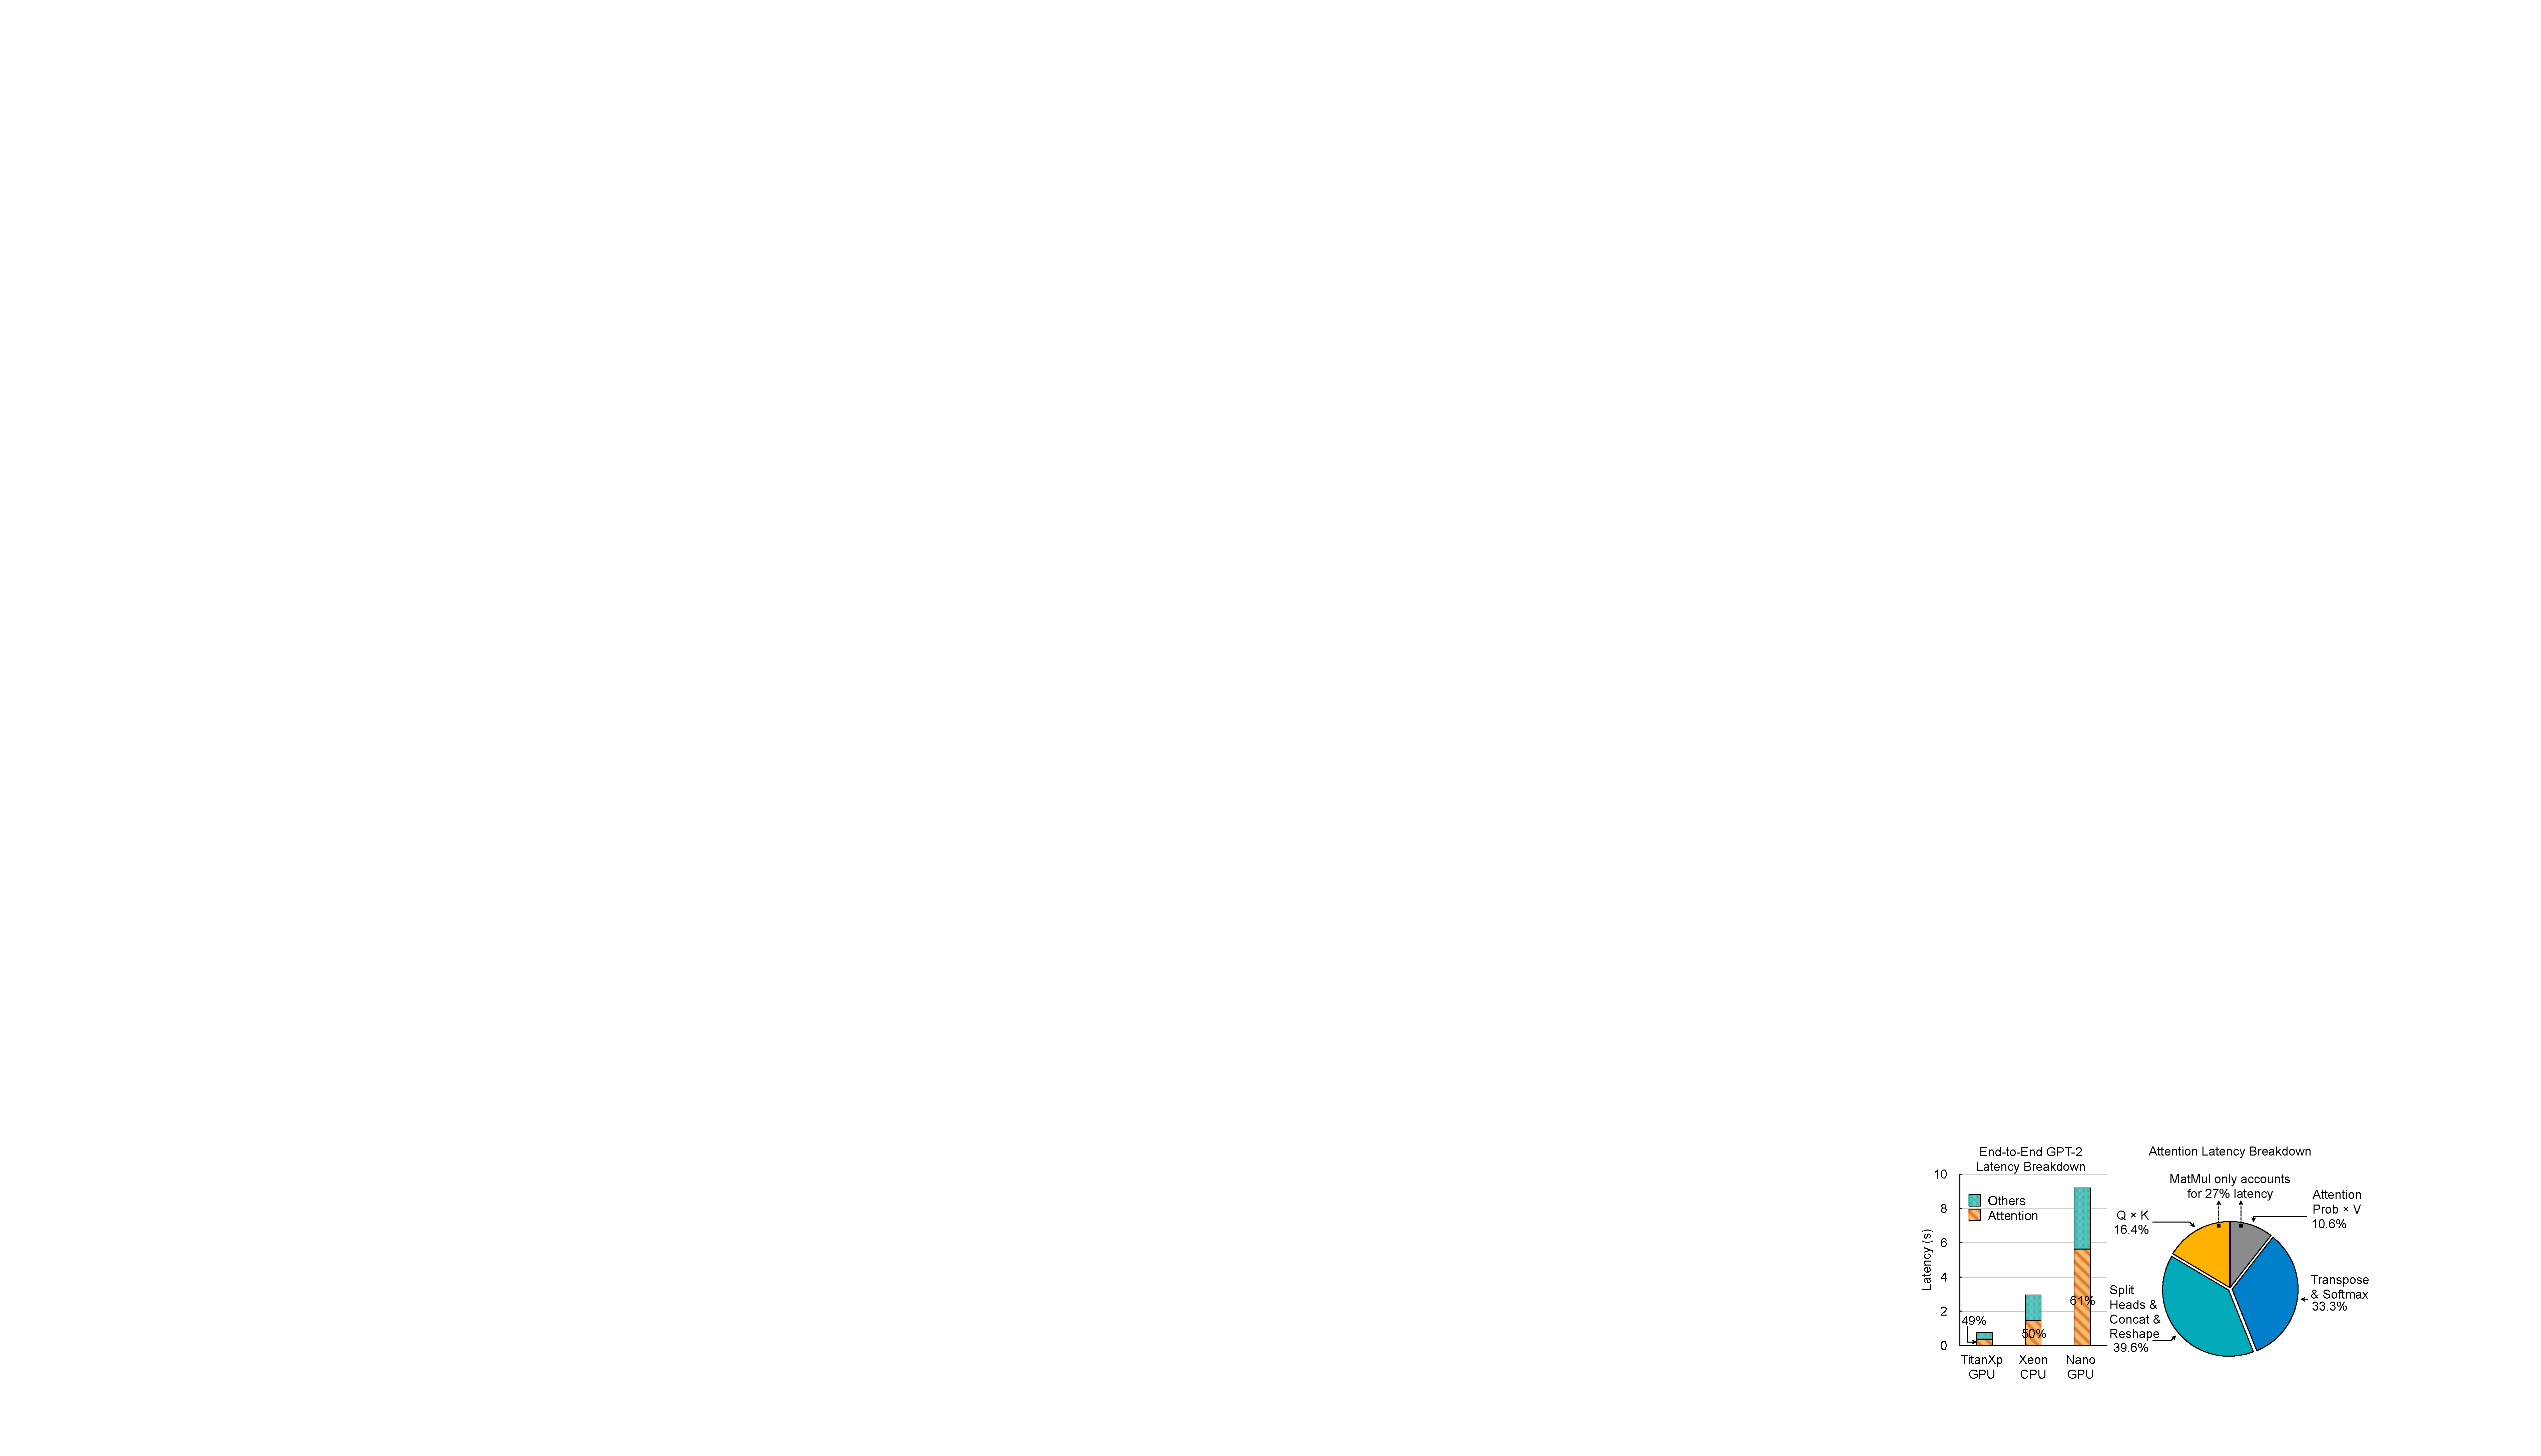
\includegraphics[width=1\columnwidth]{figures/latency_breakdown.pdf}
    \vspace{-10pt}
    \caption{End-to-End \gpttwo latency breakdown on various platforms, and attention latency breakdown on \titanxp. Attention accounts for over 50\% of total latency. Data movements account for 73\% of attention latency.}
    \vspace{-15pt}
    \label{fig:latency_breakdown}
\end{figure}


In summary, \name performs algorithm-architecture \codesign for sparse and quantized attention computing while preserving the accuracy. It makes four contributions: 
\begin{itemize}
    \item \textbf{Cascade Token Pruning} removes unimportant tokens according to the cumulative token importance scores, reducing DRAM access and computation by up to \prunegpttwodramsaving\x. 
    \item \textbf{Cascade Head Pruning} removes unimportant heads and save DRAM access and computation by another \hpdramsaving\x.
    \item \textbf{Progressive Quantization} trades a little more computation for less memory access. We change the \bitwidths of different attention heads and layers based on attention probability distribution, reducing DRAM access by \dynadramsaving\x.
    \item \textbf{Specialized High Parallelism top-k Engine} with $O(n)$ time complexity to efficiently support on-the-fly token and head selections.
\end{itemize}



We extensively evaluate \name on \numbenchmark benchmarks including GLUE set~\cite{wang-etal-2018-glue}, SQuAD\cite{rajpurkar2016squad}, Wikitext-2~\cite{merity2016pointer}, Wikitext-103~\cite{merity2016pointer}, Pen Tree Bank~\cite{marcus-etal-1993-building} and Google One-Billion Word~\cite{chelba2013one} with \bert and \gpttwo models. \name reduces DRAM access by \totaldramsaving\x with \emph{no accuracy loss}, and achieves \perfoverathree\x, \perfovermnnfast\x, \perfovertitanxp\x, \perfoverxeon\x, \perfovernano\x, \perfoverrasp\x speedup, and \eeoverathree\x, \eeovermnnfast\x, \eeovertitanxp\x, \eeoverxeon\x, \eeovernano\x, \eeoverrasp\x energy savings over \athree accelerator, \mnnfast accelerator, \titanxp, \xeon, \nano, \rasp, respectively.
